\documentclass[10pt,a4paper]{article}

\usepackage[margin=0.75cm]{geometry}
\usepackage[utf8]{inputenc}

\usepackage{amsmath}
\usepackage{amssymb}
\usepackage{biblatex}
\usepackage{textcomp}
\usepackage{gensymb}
\usepackage{paracol}
\usepackage{parskip}
\usepackage{tikz}
\usepackage{titlesec}
\usepackage{verbatim}
\usepackage{xcolor}

\titleformat{\section}[block]{\Large\bfseries\filcenter\color{black}}{\thesection}{1em}{}
\titleformat{\subsection}[block]{\bfseries\filcenter\color{black}}{\thesubsection}{1em}{}

\setlength{\columnsep}{25pt}

\tikzset{
    rounded-box/.style = {draw=blue, fill=white, thin, rectangle, rounded corners, inner sep=5pt, inner ysep=10pt},
    rounded-box-title/.style = {fill=blue, text=white, font=\bfseries},
}

\addbibresource{references.bib}

\begin{document}
\title{Differential Equations}

\section{First-Order Differential Equations}

\subsection{Numerical Methods}

\begin{paracol}{2}

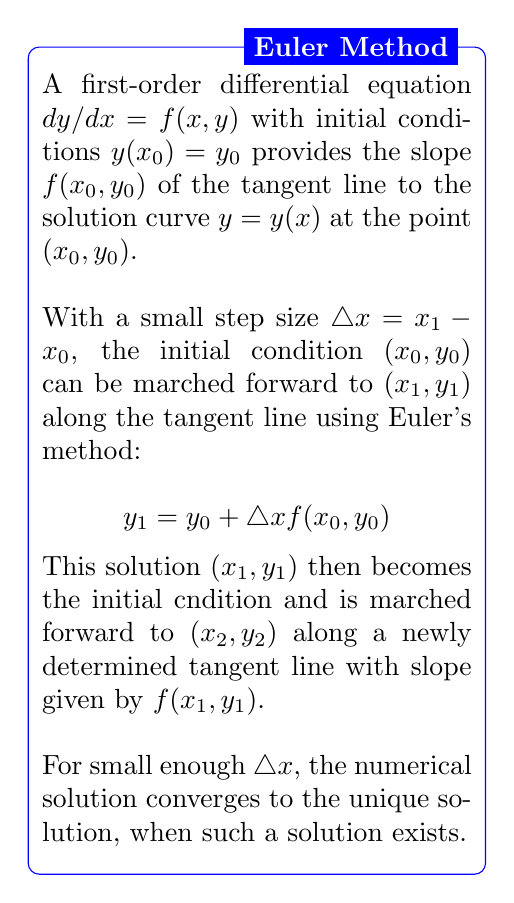
\begin{tikzpicture}
\node [rounded-box] (box){\begin{minipage}{0.45\textwidth}
    A first-order differential equation $dy/dx = f(x, y)$ with initial conditions $y(x_0) = y_0$ provides the slope $f(x_0, y_0)$ of the tangent line to the solution curve $y = y(x)$ at the point $(x_0, y_0)$. \\

    With a small step size $\triangle x = x_1 - x_0$, the initial condition $(x_0, y_0)$ can be marched forward to $(x_1, y_1)$ along the tangent line using Euler's method:

    $$y_1 = y_0 + \triangle x f(x_0, y_0)$$

    This solution $(x_1, y_1)$ then becomes the initial cndition and is marched forward to $(x_2, y_2)$ along a newly determined tangent line with slope given by $f(x_1, y_1)$. \\

    For small enough $\triangle x$, the numerical solution converges to the unique solution, when such a solution exists.
\end{minipage}};
\node[rounded-box-title, left=10pt] at (box.north east) {Euler Method};
\end{tikzpicture}

\switchcolumn

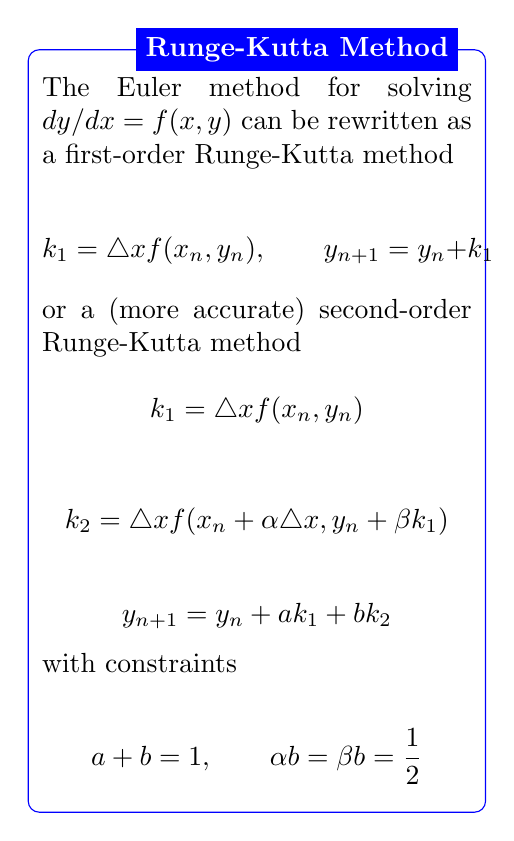
\begin{tikzpicture}
\node [rounded-box] (box){\begin{minipage}{0.45\textwidth}
    The Euler method for solving $dy/dx = f(x, y)$ can be rewritten as a first-order Runge-Kutta method

    $$k_1 = \triangle x f(x_n, y_n), \qquad y_{n+1} = y_n + k_1$$

    or a (more accurate) second-order Runge-Kutta method

    $$k_1 = \triangle x f(x_n, y_n)$$
    
    $$k_2 = \triangle x f(x_n + \alpha \triangle x, y_n + \beta k_1)$$
    
    $$y_{n+1} = y_n + a k_1 + b k_2$$

    with constraints

    \vspace{-2.5pt}

    $$a + b = 1, \qquad \alpha b = \beta b = \frac{1}{2}$$
\end{minipage}};
\node[rounded-box-title, left=10pt] at (box.north east) {Runge-Kutta Method};
\end{tikzpicture}

\end{paracol}

\subsection{Separable First-Order Equations}

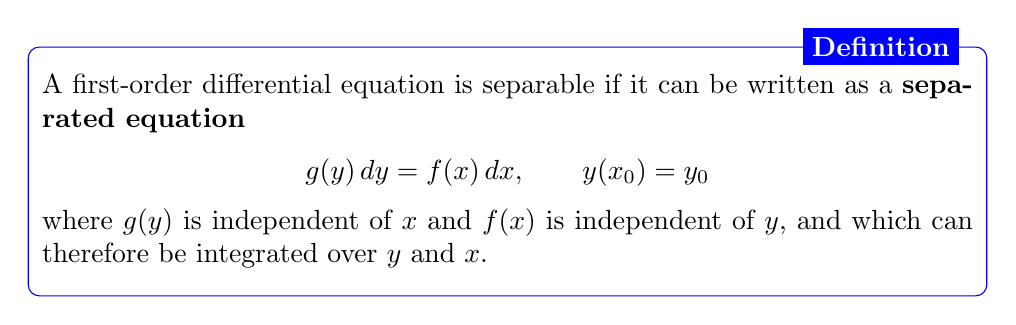
\begin{tikzpicture}
\node [rounded-box] (box){\begin{minipage}{0.975\textwidth}
    A first-order differential equation is separable if it can be written as a \textbf{separated equation}

    \vspace{-5pt}

    $$g(y) \, dy = f(x) \, dx, \qquad y(x_0) = y_0$$

    where $g(y)$ is independent of $x$ and $f(x)$ is independent of $y$, and which can therefore be integrated over $y$ and $x$.
\end{minipage}};
\node[rounded-box-title, left=10pt] at (box.north east) {Definition};
\end{tikzpicture}

\textbf{Example}: $y' + y^2 \sin(x) = 0, \quad y(0) = 1$.

\vspace{-15pt}

$$
\frac{dy}{dx} = -y^2 \sin(x)  \Rightarrow  \frac{dy}{y^2} = - \sin(x) \, dx
 \Rightarrow  \int_1^y \frac{dy}{y^2} = - \int_0^x \sin(x) \, dx
 \Rightarrow  - \frac{1}{y} \Big|_1^y = \cos(x) \Big|_0^x
 \Rightarrow  1 - \frac{1}{y} = \cos(x) - 1
 \Rightarrow  y = \frac{1}{2 - \cos(x)}
$$

\subsection{Linear First-Order Equations}

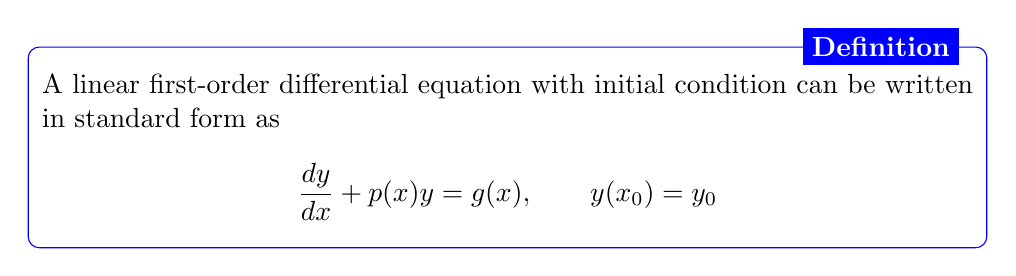
\begin{tikzpicture}
\node [rounded-box] (box){\begin{minipage}{0.975\textwidth}
    A linear first-order differential equation with initial condition can be written in standard form as

    $$\frac{dy}{dx} + p(x) y = g(x), \qquad y(x_0) = y_0$$
\end{minipage}};
\node[rounded-box-title, left=10pt] at (box.north east) {Definition};
\end{tikzpicture}

All such linear first-order equations can be integrated using an integrating factor $\mu$:

\begin{enumerate}
    \item Multiply both sides by the yet unknown function $\mu = \mu(x)$ so that $\mu(x) \Big( \frac{dy}{dx} + p(x) y \Big) = \mu(x) g(x)$

    \item Require $\mu(x)$ to satisfy the differential equation $\mu(x) \Big( \frac{dy}{dx} + p(x) y \Big) = \frac{d}{dx}(\mu(x) y)$

    \item Thus, $\frac{d}{dx}(\mu(x) y) = \mu(x) g(x)$. Using $y(x_0) = y_0$ and choosing $\mu(x_0) = 1$,

    \vspace{-10pt}

    $$\int_{x_0}^x \frac{d}{dx}(\mu(x) y) \, dx = \int_{x_0}^x \mu(x) g(x) \, dx \quad \Rightarrow \quad \mu(x) y - y_0 = \int_{x_0}^x \mu(x) g(x) \, dx \quad \Rightarrow \quad y(x) = \frac{1}{\mu(x)} \Big( y_0 + \int_{x_0}^x \mu(x) g(x) \, dx \Big)$$

    \item By the product rule, $\mu \frac{dy}{dx} + \mu p y = \frac{d\mu}{dx} y + \mu \frac{dy}{dx}$, which gives the separable differential equation

    $$\frac{d\mu}{dx} = p(x) \mu, \qquad \mu(x_0) = 1 \qquad \text{which can be integrated to obtain} \qquad \mu(x) = e^{\int_{x_0}^x p(x) \, dx}$$

    \item Combining the previous two steps solves the differential equation.
\end{enumerate}

\textbf{Example}: Consider the inseparable linear equation $\frac{dy}{dx} + 2 y = e^{-x}, \quad y(0) = \frac{3}{4}$. Let $p(x) = 2, g(x) = e^{-x}$. Then

$$\mu(x) = e^{\int_0^x 2 \, dx} = e^{2x}, \qquad y(x) = e^{-2x} \Big( \frac{3}{4} + \int_0^x e^{2x} e^{-x} \, dx \Big) = e^{-2x} \Big( \frac{3}{4} + (e^x - 1) \Big) = e^{-x} \Big( 1 - \frac{1}{4} e^{-x} \Big)$$

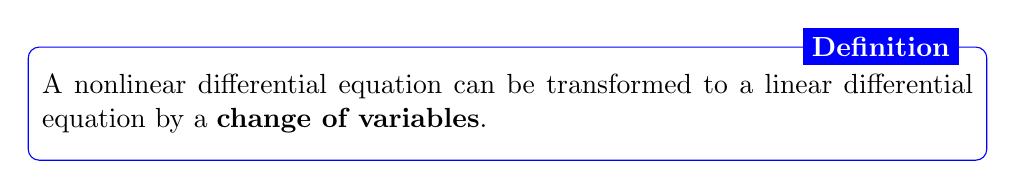
\begin{tikzpicture}
\node [rounded-box] (box){\begin{minipage}{0.975\textwidth}
    A nonlinear differential equation can be transformed to a linear differential equation by a \textbf{change of variables}.
\end{minipage}};
\node[rounded-box-title, left=10pt] at (box.north east) {Definition};
\end{tikzpicture}

\textbf{Example}: Consider the nonlinear differential equation $\frac{dx}{dt} = x (1-x)$.

\begin{paracol}{2}

Let $z = \frac{1}{x}$. Then

$$x = \frac{1}{z}, \qquad \frac{dx}{dt} = \frac{dx}{dz} \frac{dz}{dt} = - \frac{1}{z^2} \frac{dz}{dt}$$

\switchcolumn

Thus,

\vspace{-10pt}

$$
\frac{dx}{dt} = x (1-x)
\quad \Rightarrow \quad
- \frac{1}{z^2} \frac{dz}{dt} = \frac{1}{z} \Big( 1 - \frac{1}{z}\Big)
\quad \Rightarrow \quad
\frac{dz}{dt} + z = 1
$$

\end{paracol}

\subsection{Applications}

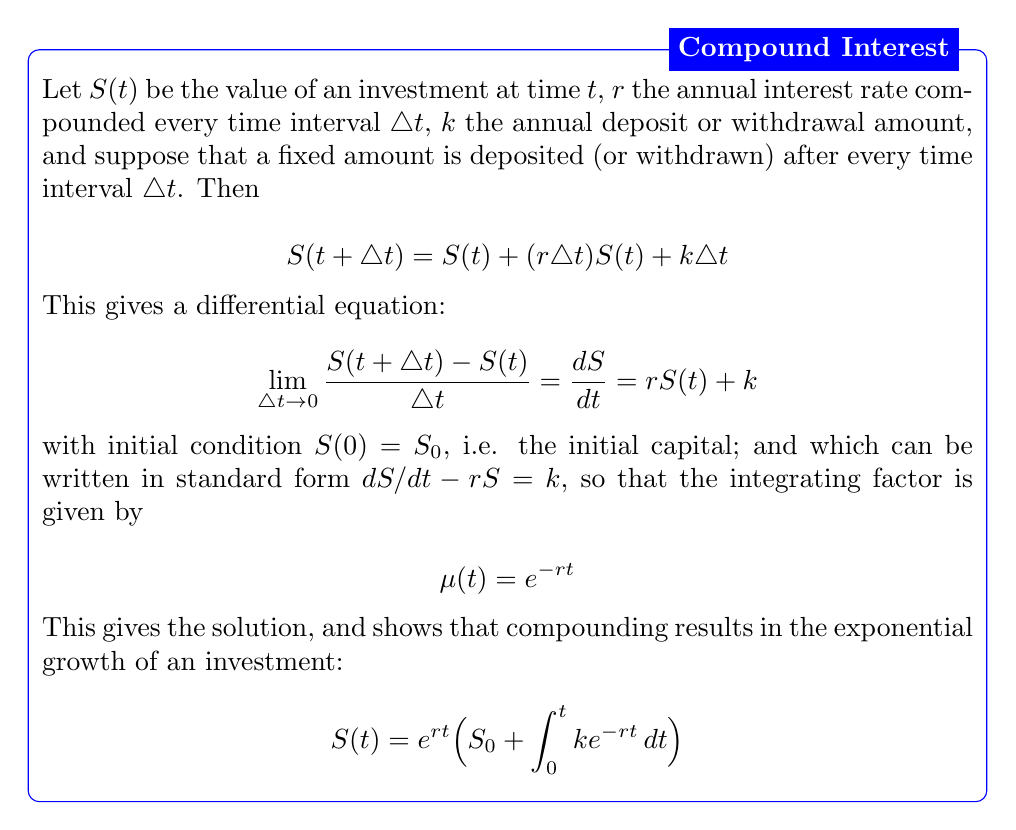
\begin{tikzpicture}
\node [rounded-box] (box){\begin{minipage}{0.975\textwidth}
    Let $S(t)$ be the value of an investment at time $t$, $r$ the annual interest rate compounded every time interval $\triangle t$, $k$ the annual deposit or withdrawal amount, and suppose that a fixed amount is deposited (or withdrawn) after every time interval $\triangle t$. Then

    $$S(t + \triangle t) = S(t) + (r \triangle t) S(t) + k \triangle t$$

    This gives a differential equation:

    $$\lim_{\triangle t \rightarrow 0} \frac{S(t + \triangle t) - S(t)}{\triangle t} = \frac{dS}{dt} = r S(t) + k$$

    with initial condition $S(0) = S_0$, i.e. the initial capital; and which can be written in standard form $dS/dt - rS = k$, so that the integrating factor is given by

    $$\mu(t) = e^{-rt}$$

    This gives the solution, and shows that compounding results in the exponential growth of an investment:

    $$S(t) = e^{rt} \Big( S_0 + \int_0^t k e^{-rt} \, dt \Big)$$
\end{minipage}};
\node[rounded-box-title, left=10pt] at (box.north east) {Compound Interest};
\end{tikzpicture}

\subsection{Modelling with Differential Equations}

\begin{paracol}{2}

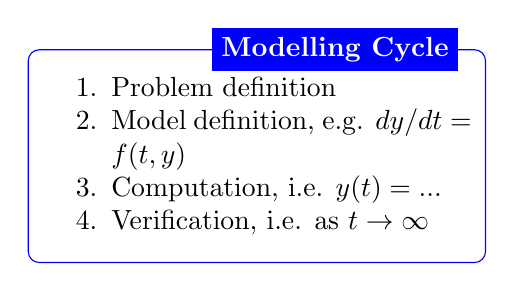
\begin{tikzpicture}
\node [rounded-box] (box){\begin{minipage}{0.45\textwidth}
    \begin{enumerate}
        \item Problem definition
        \item Model definition, e.g. $dy / dt = f(t, y)$
        \item Computation, i.e. $y(t) = ...$
        \item Verification, i.e. as $t \rightarrow \infty$
    \end{enumerate}
\end{minipage}};
\node[rounded-box-title, left=10pt] at (box.north east) {Modelling Cycle};
\end{tikzpicture}

\textbf{Example}: You want to breed rainbowfish to sell to pet stores. You start with a nice big aquarium and 30 fish, half of them male, half of them female. You want to predict the number of fish after a number of days, to see how many you can sell.

In this particular case, we have the balance equation:

$$\triangle P = P(t + \triangle t) - P(t) = 0.7 P(t) \triangle t$$

Which results in the differential equation for the problem:

$$\frac{dP}{dt} = \lim_{\triangle t \rightarrow 0} \frac{\triangle P}{\triangle t} = = 0.7 P(t), \quad P(0) = 30$$

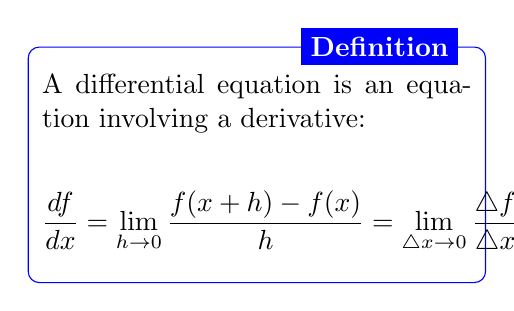
\begin{tikzpicture}
\node [rounded-box] (box){\begin{minipage}{0.45\textwidth}
    A differential equation is an equation involving a derivative:

    $$\frac{df}{dx} = \lim_{h \rightarrow 0} \frac{f(x + h) - f(x)}{h} = \lim_{\triangle x \rightarrow 0} \frac{\triangle f}{\triangle x}$$
\end{minipage}};
\node[rounded-box-title, left=10pt] at (box.north east) {Definition};
\end{tikzpicture}

\switchcolumn

If you use only words to describe the differential equation you would say: "The derivative of the function equals a multiple of the function." So the solution to the differential equation should be a function with this property.

\textbf{Example} continued: Let $P(t) = c e^{kt}$.

Given the differential equation and its initial condition, $k = 0.7$, and $c = 30$. Thus, the solution is $P(t) = 30 e^{0.7 t}$. (This simplified model only considers a birth rate $b = 0.7$ but not a death rate $d$.)

\textbf{Example} continued: A more realistic model is given by a model with \textbf{bounded growth}:

$$\frac{dP}{dt} = 0.7 P \Big(1 - \frac{P}{750} \Big) - 20, P(0) = 30$$

The differential equation for the rainbowfish that we have now, could still be solved by hand. It would give you the analytical solution, which is exact. In practice, for a more complicated model, you would probably use a numerical method like Euler's Method to approximate the solution.

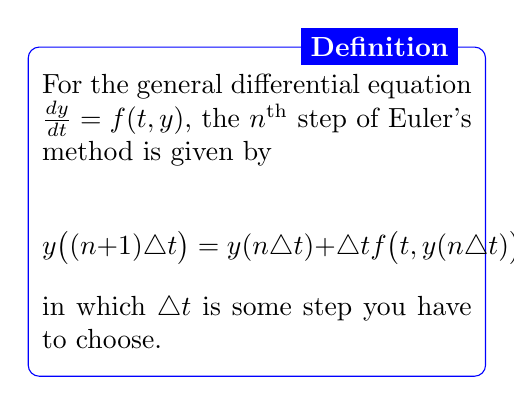
\begin{tikzpicture}
\node [rounded-box] (box){\begin{minipage}{0.45\textwidth}
    For the general differential equation $\frac{dy}{dt} = f(t, y)$, the $n^\text{th}$ step of Euler's method is given by

    $$y\big((n+1) \triangle t\big) = y(n \triangle t) + \triangle t f\big(t, y(n \triangle t)\big)$$

    in which $\triangle t$ is some step you have to choose.
\end{minipage}};
\node[rounded-box-title, left=10pt] at (box.north east) {Definition};
\end{tikzpicture}

\end{paracol}
 \newpage
\section{Homogeneous Linear Differential Equations}

\subsection{Numerical Methods}

Most higher-order ODEs are usually solved numerically.

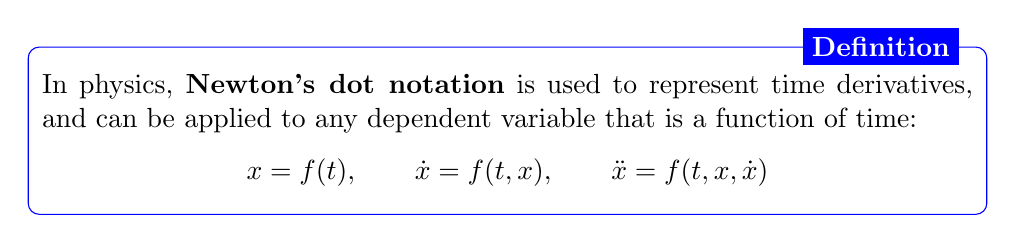
\begin{tikzpicture}
\node [rounded-box] (box){\begin{minipage}{0.975\textwidth}
    In physics, \textbf{Newton's dot notation} is used to represent time derivatives, and can be applied to any dependent variable that is a function of time:

    \vspace{-5pt}

    $$x = f(t), \qquad \dot{x} = f(t, x), \qquad \ddot{x} = f(t, x, \dot{x})$$
\end{minipage}};
\node[rounded-box-title, left=10pt] at (box.north east) {Definition};
\end{tikzpicture}

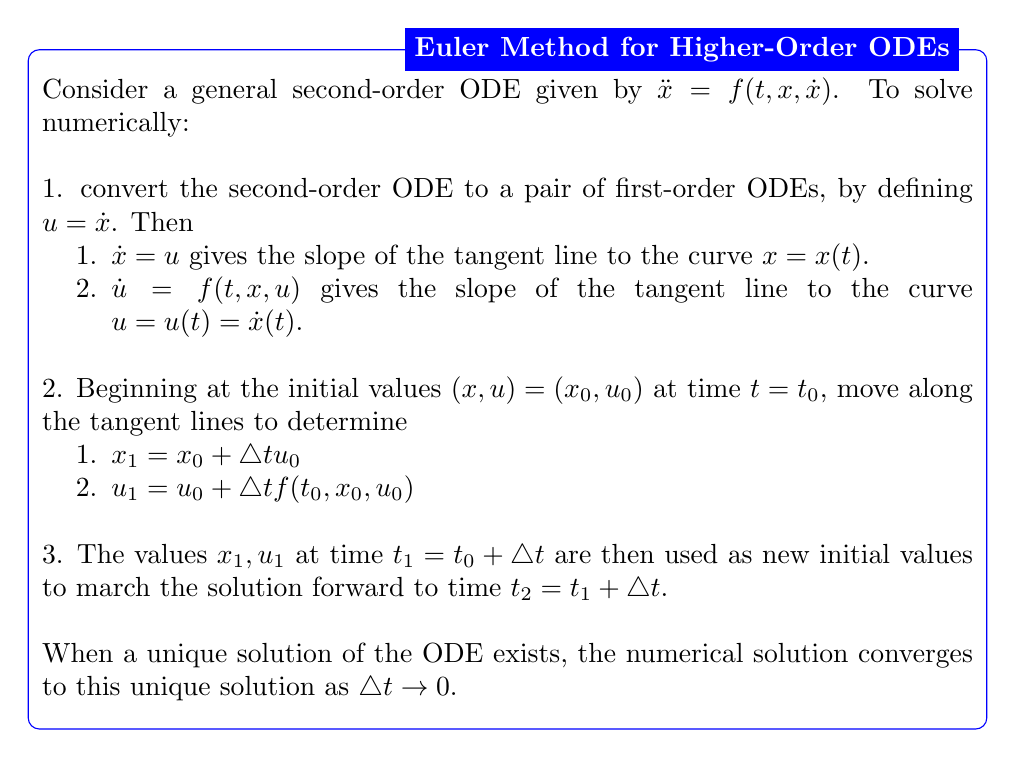
\begin{tikzpicture}
\node [rounded-box] (box){\begin{minipage}{0.975\textwidth}
    Consider a general second-order ODE given by $\ddot{x} = f(t, x, \dot{x})$. To solve numerically: \\

    1. convert the second-order ODE to a pair of first-order ODEs, by defining $u = \dot{x}$. Then

    \begin{enumerate}
        \item $\dot{x} = u$ gives the slope of the tangent line to the curve $x = x(t)$.

        \item $\dot{u} = f(t, x, u)$ gives the slope of the tangent line to the curve $u = u(t) = \dot{x}(t)$. \\
    \end{enumerate}

    2. Beginning at the initial values $(x, u) = (x_0, u_0)$ at time $t = t_0$, move along the tangent lines to determine

    \begin{enumerate}
        \item $x_1 = x_0 + \triangle t u_0$

        \item $u_1 = u_0 + \triangle t f(t_0, x_0, u_0)$ \\
    \end{enumerate}

    3. The values $x_1, u_1$ at time $t_1 = t_0 + \triangle t$ are then used as new initial values to march the solution forward to time $t_2 = t_1 + \triangle t$. \\

    When a unique solution of the ODE exists, the numerical solution converges to this unique solution as $\triangle t \rightarrow 0$.
\end{minipage}};
\node[rounded-box-title, left=10pt] at (box.north east) {Euler Method for Higher-Order ODEs};
\end{tikzpicture}

\subsection{Theory}

\begin{paracol}{2}

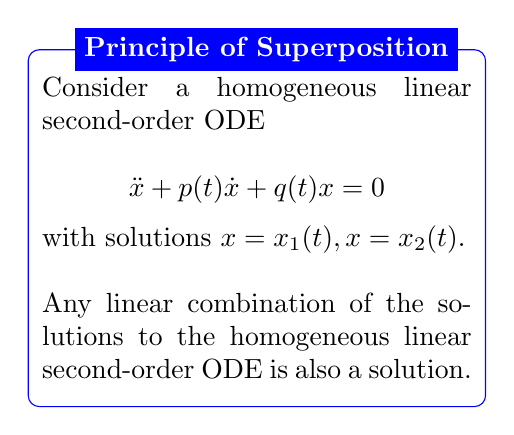
\begin{tikzpicture}
\node [rounded-box] (box){\begin{minipage}{0.45\textwidth}
    Consider a homogeneous linear second-order ODE

    $$\ddot{x} + p(t) \dot{x} + q(t) x = 0$$

    with solutions $x = x_1(t), x = x_2(t)$. \\
    
    Any linear combination of the solutions to the homogeneous linear second-order ODE is also a solution.
\end{minipage}};
\node[rounded-box-title, left=10pt] at (box.north east) {Principle of Superposition};
\end{tikzpicture}

\switchcolumn

\vspace{10pt}

\textbf{Proof}:

\vspace{-15pt}

\begin{align*}
    \ddot{x} + & p(t) \dot{x} + q(t) x \\
    & = c_1 \ddot{x}_1 + c_2 \ddot{x}_2 + p(c_1 \dot{x}_1 + c_2 \dot{x}_2) + q(c_1 x_1 + c_2 x_2) \\
    & = c_1 (\ddot{x}_1 + p \dot{x}_1 + q x_1) + c_2 (\ddot{x}_2 + p \dot{x}_2 + q x_2) \\
    & = c_1 \times 0 + c_2 \times 0, \text{ since } x_1, x_2 \text{ are solutions} \\
    & = 0
\end{align*}

\end{paracol}

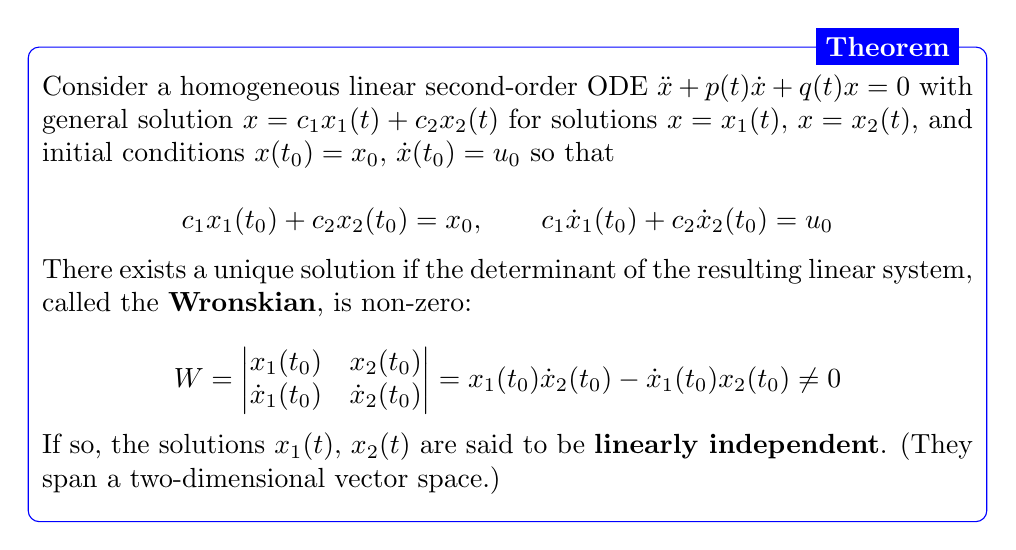
\begin{tikzpicture}
\node [rounded-box] (box){\begin{minipage}{0.975\textwidth}
    Consider a homogeneous linear second-order ODE $\ddot{x} + p(t) \dot{x} + q(t) x = 0$ with general solution $x = c_1 x_1(t) + c_2 x_2(t)$ for solutions $x = x_1(t), \, x = x_2(t)$, and initial conditions $x(t_0) = x_0, \, \dot{x}(t_0) = u_0$ so that

    $$c_1 x_1(t_0) + c_2 x_2(t_0) = x_0, \qquad c_1 \dot{x}_1(t_0) + c_2 \dot{x}_2(t_0) = u_0$$

    There exists a unique solution if the determinant of the resulting linear system, called the \textbf{Wronskian}, is non-zero:

    $$W = \begin{vmatrix}
        x_1(t_0) & x_2(t_0) \\
        \dot{x}_1(t_0) & \dot{x}_2(t_0)
    \end{vmatrix} = x_1(t_0) \dot{x}_2(t_0) - \dot{x}_1(t_0) x_2(t_0) \neq 0$$

    If so, the solutions $x_1(t), \, x_2(t)$ are said to be \textbf{linearly independent}. (They span a two-dimensional vector space.)
\end{minipage}};
\node[rounded-box-title, left=10pt] at (box.north east) {Theorem};
\end{tikzpicture}

\textbf{Example}: Given a homogeneous linear second-order ODE with solutions $x_1(t) = \cos(\omega t), \, x_2(t) = \sin(\omega t), \, \omega \neq 0$, the Wronskian $W = (\cos \omega t) (\omega \cos \omega t) - (- \omega \sin \omega t) (\sin \omega t) = \omega \neq 0$ for all $t$.

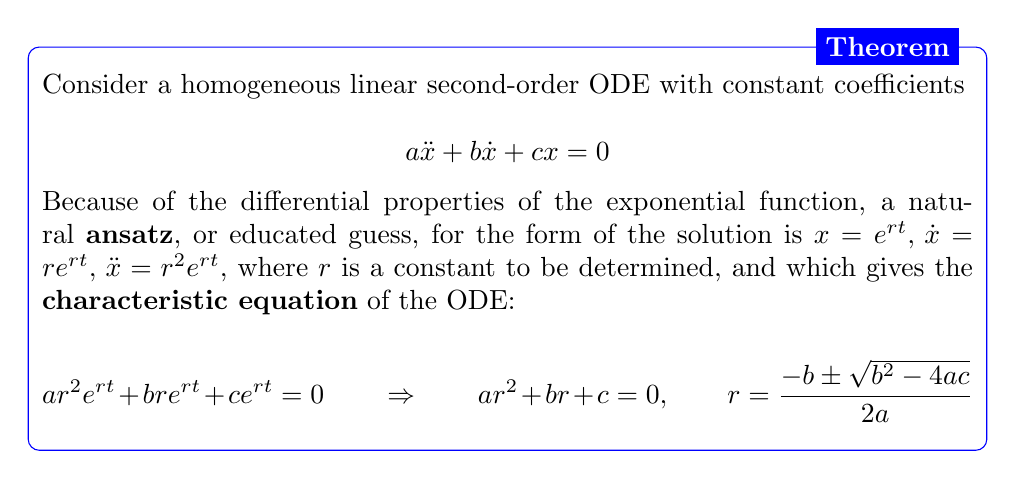
\begin{tikzpicture}
\node [rounded-box] (box){\begin{minipage}{0.975\textwidth}
    Consider a homogeneous linear second-order ODE with constant coefficients

    $$a \ddot{x} + b \dot{x} + c x = 0$$

    Because of the differential properties of the exponential function, a natural \textbf{ansatz}, or educated guess, for the form of the solution is $x = e^{rt}, \, \dot{x} = r e^{rt}, \, \ddot{x} = r^2 e^{rt}$, where $r$ is a constant to be determined, and which gives the \textbf{characteristic equation} of the ODE:

    \vspace{-5pt}

    $$a r^2 e^{rt} + b r e^{rt} + c e^{rt} = 0 \qquad \Rightarrow \qquad a r^2 + b r + c = 0, \qquad r = \frac{-b \pm \sqrt{b^2 - 4 a c}}{2a}$$
\end{minipage}};
\node[rounded-box-title, left=10pt] at (box.north east) {Theorem};
\end{tikzpicture}

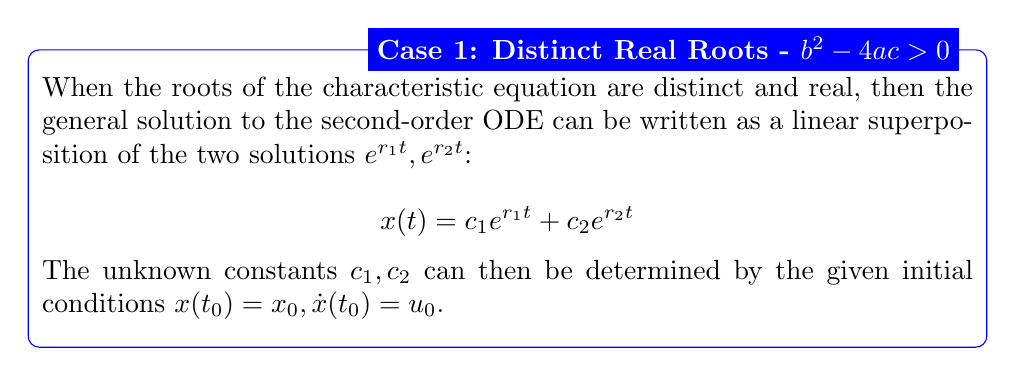
\begin{tikzpicture}
\node [rounded-box] (box){\begin{minipage}{0.975\textwidth}
    When the roots of the characteristic equation are distinct and real, then the general solution to the second-order ODE can be written as a linear superposition of the two solutions $e^{r_1 t}, e^{r_2 t}$:
    
    $$x(t) = c_1 e^{r_1 t} + c_2 e^{r_2 t}$$
    
    The unknown constants $c_1, c_2$ can then be determined by the given initial conditions $x(t_0) = x_0, \dot{x}(t_0) = u_0$.
\end{minipage}};
\node[rounded-box-title, left=10pt] at (box.north east) {Case 1: Distinct Real Roots - $b^2 - 4 a c > 0$};
\end{tikzpicture}

\textbf{Example}: $\ddot{x} + 5 \dot{x} + 6 x = 0, \, x(0) = 2, \, \dot{x}(0) = 3$

Ansatz $x = e^{rt}$ gives characteristic equation $r^2 + 5r + 6 = 0$ which factors to $(r+3)(r+2) = 0$.

The general solution to the ODE is therefore $x(t) = c_1 e^{-2t} + c_2 e^{-3t}$, and by differentiation $\dot{x}(t) = - 2 c_1 c^{-2t} - 3 c_2 e^{3t}$.

Plugging in the initial conditions gives $c_1 + c_2 = 2, \, -2 c_1 - 3 c_2 = 3$ with solution $c_1 = 9, \, c_2 = -7$.

Therefore, the unique solution that satisfies the ODE and its initial conditions is

$$x(t) = 9 e^{-2t} - 7 e^{-3t} = 9 e^{-2t} \Big( 1 - \frac{7}{9} e^{-t} \Big)$$

\vspace{10pt}

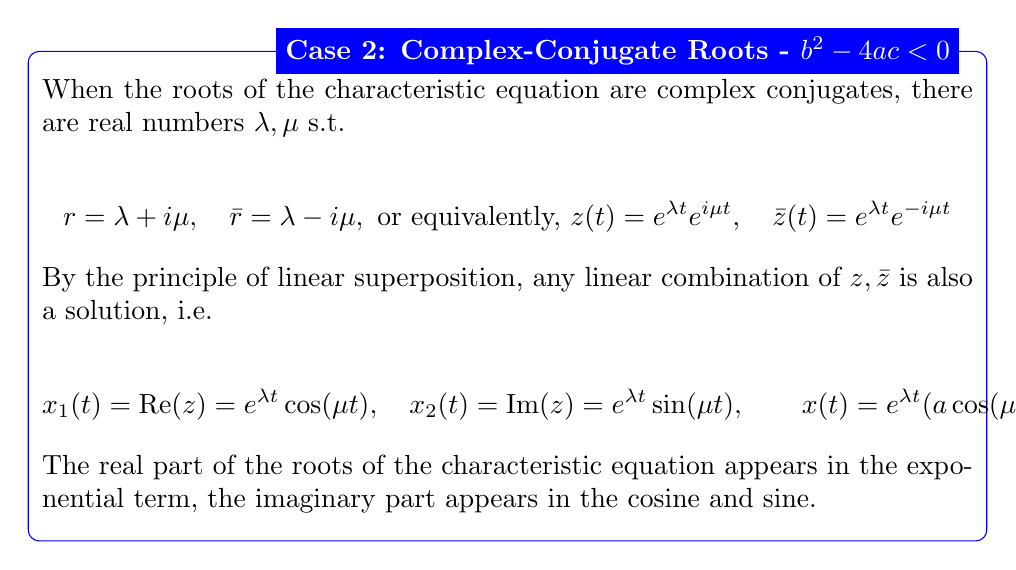
\begin{tikzpicture}
\node [rounded-box] (box){\begin{minipage}{0.975\textwidth}
    When the roots of the characteristic equation are complex conjugates, there are real numbers $\lambda, \mu$ s.t.
    
    $$r = \lambda + i \mu, \quad \bar{r} = \lambda - i \mu, \text{ or equivalently, } z(t) = e^{\lambda t} e^{i \mu t}, \quad \bar{z}(t) = e^{\lambda t} e^{-i \mu t}$$
    
    By the principle of linear superposition, any linear combination of $z, \bar{z}$ is also a solution, i.e.
    
    $$x_1(t) = \text{Re}(z) = e^{\lambda t} \cos(\mu t), \quad x_2(t) = \text{Im}(z) = e^{\lambda t} \sin(\mu t), \qquad x(t) = e^{\lambda t} (a \cos(\mu t) + b \sin(\mu t))$$
    
    The real part of the roots of the characteristic equation appears in the exponential term, the imaginary part appears in the cosine and sine.
\end{minipage}};
\node[rounded-box-title, left=10pt] at (box.north east) {Case 2: Complex-Conjugate Roots - $b^2 - 4 a c < 0$};
\end{tikzpicture}

\textbf{Example}: $\ddot{x} + \dot{x} + x = 0, \, x(0) = 1, \, \dot{x}(0) = 0$ with characteristic equation $r^2 + r + 1 = 0$ and roots $r = - \frac{1}{2} \pm i \frac{\sqrt{3}}{2}$

The general solution to the ODE is therefore $x(t) = e^{-t/2} \Bigg( a \cos\Big(\frac{\sqrt{3}}{2}t\Big) + b \sin\Big(\frac{\sqrt{3}}{2}t\Big) \Bigg)$.

The derivative is $\dot{x}(t) = -\frac{1}{2} e^{-t/2} \Bigg( a \cos\Big(\frac{\sqrt{3}}{2}t\Big) + b \sin\Big(\frac{\sqrt{3}}{2}t\Big) \Bigg) + \frac{\sqrt{3}}{2} e^{-t/2} \Bigg( -a \sin\Big(\frac{\sqrt{3}}{2}t\Big) + b \cos\Big(\frac{\sqrt{3}}{2}t\Big) \Bigg)$.

Plugging in the initial conditions gives $a = 1, \, -\frac{1}{2} a + \frac{\sqrt{3}}{2} b = 0$ with solution $a = 1, \, b = \sqrt{3} / 3$.

Therefore, the unique solution that satisfies the ODE and its initial conditions is

$$x(t) = e^{-t/2} \Bigg( \cos\Big( \frac{\sqrt{3}}{2}t \Big) + \frac{\sqrt{3}}{3} \sin\Big( \frac{\sqrt{3}}{2}t \Big) \Bigg)$$

\vspace{10pt}

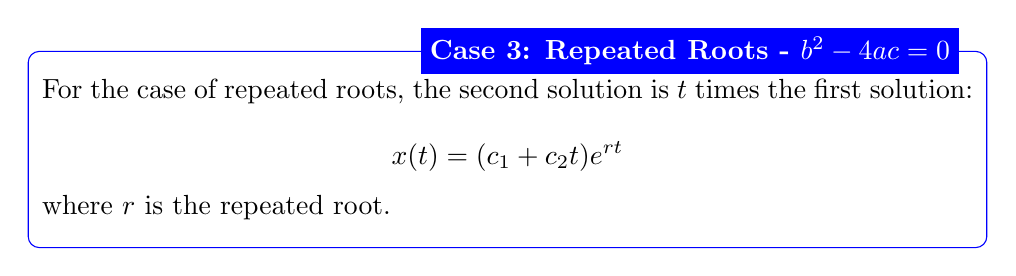
\begin{tikzpicture}
\node [rounded-box] (box){\begin{minipage}{0.975\textwidth}
    For the case of repeated roots, the second solution is $t$ times the first solution:
    
    $$x(t) = (c_1 + c_2 t) e^{rt}$$

    where $r$ is the repeated root.
\end{minipage}};
\node[rounded-box-title, left=10pt] at (box.north east) {Case 3: Repeated Roots - $b^2 - 4 a c = 0$};
\end{tikzpicture}

\textbf{Example}: $\ddot{x} + 2 \dot{x} + x = 0, \, x(0) = 1, \, \dot{x}(0) = 0$

The characteristic equation $r^2 + 2r + 1 = (r + 1)^2 = 0$ has a repeated root $r = 1$.

The general solution to the ODE is therefore $x(t) = (c_1 + c_2 t) e^{-t}, \, \dot{x}(t) = (c_2 - c_1 - c_2 t) e^{-t}$.

Plugging in the initial conditions gives $c_1 = 1, \, c_2 - c_1 = 0$ with solution $c_1 = c_2 = 1$.

Therefore, the unique solution that satisfies the ODE and its initial conditions is

$$x(t) = (1 + t) e^{-t}$$
 \newpage
\section{Inhomogeneous Linear Differential Equations}

We now add an inhomogeneous term to the second-order ode with constant coefficients. The in-homogeneous term may be an exponential, a sine or cosine, or a polynomial. A general solution will be the sum of a homogeneous and particular solution.

\subsection{Theory}

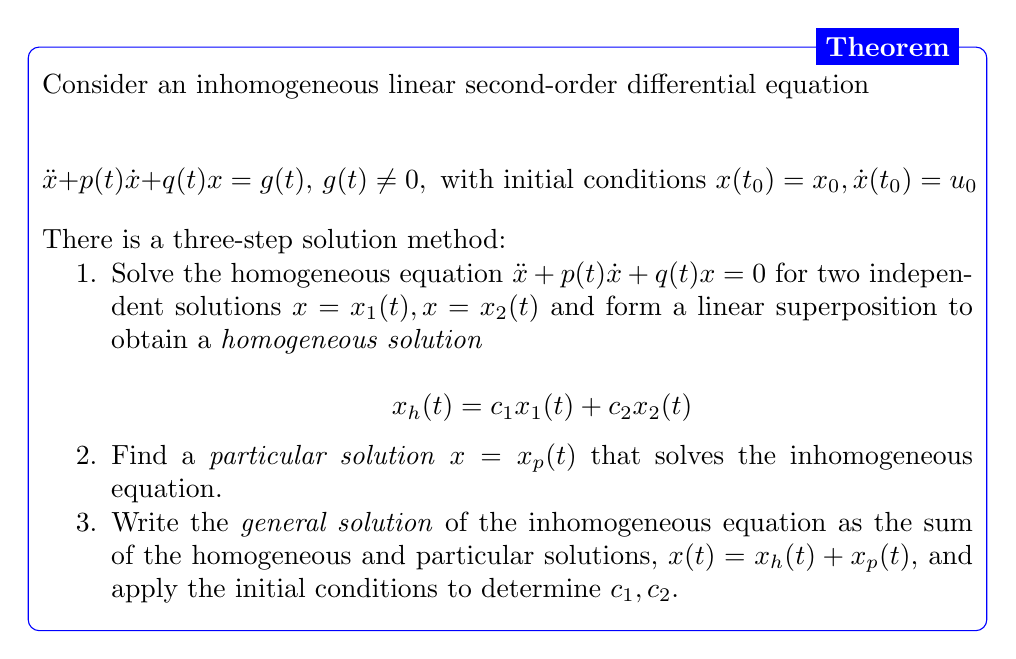
\begin{tikzpicture}
\node [rounded-box] (box){\begin{minipage}{0.975\textwidth}
    Consider an inhomogeneous linear second-order differential equation

    $$\ddot{x} + p(t) \dot{x} + q(t) x = g(t), \, g(t) \neq 0, \text{ with initial conditions } x(t_0) = x_0, \dot{x}(t_0) = u_0$$

    There is a three-step solution method:

    \begin{enumerate}
        \item Solve the homogeneous equation $\ddot{x} + p(t) \dot{x} + q(t) x = 0$ for two independent solutions $x = x_1(t), x = x_2(t)$ and form a linear superposition to obtain a \textit{homogeneous solution}

        $$x_h(t) = c_1 x_1(t) + c_2 x_2(t)$$

        \item Find a \textit{particular solution} $x = x_p(t)$ that solves the inhomogeneous equation.

        \item Write the \textit{general solution} of the inhomogeneous equation as the sum of the homogeneous and particular solutions, $x(t) = x_h(t) + x_p(t)$, and apply the initial conditions to determine  $c_1, c_2$.
    \end{enumerate}
\end{minipage}};
\node[rounded-box-title, left=10pt] at (box.north east) {Theorem};
\end{tikzpicture}

Note: The two free constants in $x_h$ can be used to satisfy the two initial conditions because the sum of the homogeneous and particular soltuions solve the ODE, by linearity:

\begin{align*}
    \ddot{x} + p \dot{x} + q x & = \frac{d^2}{dt^2}(x_h + x_p) + p \frac{d}{dt}(x_h + x_p) + q (x_h + x_p) \\
    & = (\ddot{x}_h + p \dot{x}_h + q x_h) + (\ddot{x}_p + p \dot{x}_p + q x_p) \\
    & = 0 + g = g
\end{align*}

\subsection{Particular Solutions for Exponential, Sine / Cosine and Polynomial Inhomogeneous Terms}

\begin{paracol}{2}

\textbf{Example}: $\ddot{x} - 3 \dot{x} - 4 x = 3 e^{2t}, x(0) = 1, \dot{x}(0) = 0$

\begin{enumerate}
    \item The characteristic equation of the homogeneous equation is $r^2 - 3r - 4 = (r-4) (r+1) = 0$ so that $x_h(t) = c_1 e^{4t} + c_2 e^{-t}$.
    
    \item For the inhomogeneous solution, an Ansatz such that the exponential function cancels, $x(t) = A e^{2t}$, where $A$ is an undetermined coefficient, gives $4A - 6A - 4A = 3$ and consequently $A = -1/2$. Obtaining a solution for $A$ independent of $t$ justifies the Ansatz.
    
    \item Plugging the initial conditions in $x(t) = x_h(t) + x_p(t) = c_1 e^{4t}+ c_2 e^{-t} - \frac{1}{2} e^{2t}, \quad \dot{x}(t) = \dot{x}_h(t) + \dot{x}_p(t) = 4 c_1 e^{4t} - c_2 e^{-t} - e^{2t}$ gives $c_1 + c_2 = 3/2, \quad 4 c_1 - c_2 = 1$ with solution $c_1 = 1/2, c_2 = 1$.
\end{enumerate}

The solution is

$$x(t) = \frac{1}{2} e^{4t} - \frac{1}{2} e^{2t} - e^{-t} = \frac{1}{2} e^{4t} \big( 1 - e^{-2t} + 2 e^{-5t} \big)$$

\textbf{Example}: $\ddot{x} + \dot{x} - 2x = t^2$

The Ansatz should be a polynomial in $t$ of the same order as the inhomogeneous term, i.e. $x(t) = At^2 + Bt + C$.

This gives $2A + (2At + B) - 2(At^2 + Bt + C) = t^2$, or $-2At^2 + 2(A - B)t + (2A + B - 2C)t^0 = t^2$.

Equating powers of $t$, $-2A = 1, \quad 2(A-B) = 0, \quad 2A + B - 2C = 0$, gives $A = -\frac{1}{2}, \quad B = -\frac{1}{2}, C = -\frac{3}{4}$.

The particular solution is

$$x_p(t) = - \frac{1}{2}t^2 - \frac{1}{2}t - \frac{3}{4}$$

\switchcolumn

\textbf{Example}: $\ddot{x} - 3 \dot{x} - 4x = 2 \sin(t)$

\textbf{Approach 1}: Ansatz $x(t) = A \cos(t) + B \sin(t)$

The cosine term is required because it is the derivative of sine.

Substituting in the differential equation gives $(- A \cos(t)) - 3(-A \sin(t) + B \cos(t)) - 4(A \cos(t) + B \sin(t)) = 2 \sin(t)$.

Regrouping terms gives $-(5A + 3B) \cos(t) + (3A - 5B) \sin(t) = 2 \sin(t)$.

This equation is valid for all $t$, and in particular for $t = 0, t = \pi / 2$ for which the sine and cosine functions vanish. For these two values of $t$, $5A + 3B = 0, \quad 3A - 5B = 2$, which gives $A = 3/17, B = -5/17$.

The particular solution is

$$x_p = \frac{1}{17} (3 \cos(t) - 5 \sin(t))$$

\textbf{Approach 2}: Converting the sine inhomogeneous term to an exponential term, given the relation $e^{it} = \cos(t) + i \sin(t)$.

That is, sine is the imaginary part of complex function $z = z(t)$: $\sin(t) = \text{Im}\{e^{it}\}$. Therefore, $\ddot{z} - 3 \dot{z} - 4 z = 2 e^{it}$, where $x = \text{Im}\{z\}$ satisfies the original differential equation for $x$.

Substituting the Ansatz $z(t) = C e^{it}$, where $C$ is a complex constant, and using the fact that $i^2 = -1$, gives $-C -3iC - 4C = 2$ with solution $C = \frac{-2}{5+3i} = \frac{-5+3i}{17}$.

\begin{align*}
    x_p = \text{Im}\{z_p\} & = \text{Im}\Big\{ \frac{1}{17} (-5 + 3i) (\cos(t) + i \sin(t)) \Big\} \\
    & = \frac{1}{17} (3 \cos(t) - 5 \sin(t))
\end{align*}

\end{paracol}
 \newpage
\section{The Laplace Transform and Series Solution Methods}

\subsection{The Laplace Transform Method}

\begin{paracol}{2}

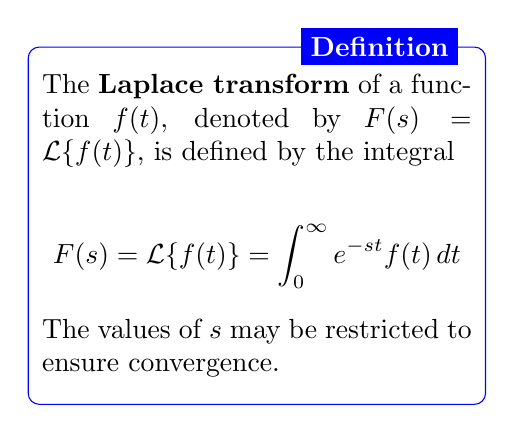
\begin{tikzpicture}
\node [rounded-box] (box){\begin{minipage}{0.45\textwidth}
    The \textbf{Laplace transform} of a function $f(t)$, denoted by $F(s) = \mathcal{L}\{ f(t) \}$, is defined by the integral

    $$F(s) = \mathcal{L}\{ f(t) \} = \int_0^\infty e^{-st} f(t) \, dt$$

    The values of $s$ may be restricted to ensure convergence.
\end{minipage}};
\node[rounded-box-title, left=10pt] at (box.north east) {Definition};
\end{tikzpicture}

\switchcolumn

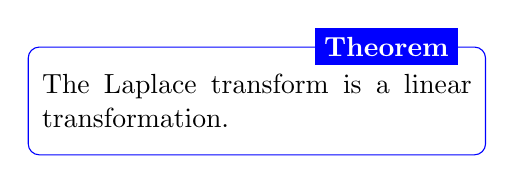
\begin{tikzpicture}
\node [rounded-box] (box){\begin{minipage}{0.45\textwidth}
    The Laplace transform is a linear transformation.
\end{minipage}};
\node[rounded-box-title, left=10pt] at (box.north east) {Theorem};
\end{tikzpicture}

\textbf{Proof}:

\begin{align*}
    & \mathcal{L}\{ c_1 f_1(t) + c_2 f_2(t) \} = \int_0^\infty e^{-st} (c_1 f_1(t) + c_2 f_2(t)) \, dt \\
    & = c_1 \int_0^\infty e^{-st} f_1(t) \, dt + c_2 \int_0^\infty e^{-st} f_2(t) \, dt \\
    & = c_1 \mathcal{L}\{ f_1(t) \} + c_2 \mathcal{L}\{ f_2(t) \}
\end{align*}

\switchcolumn

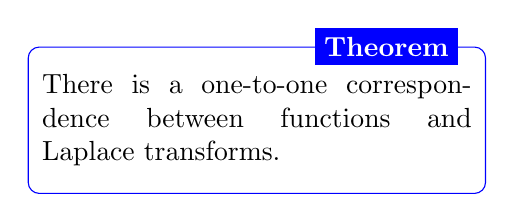
\begin{tikzpicture}
\node [rounded-box] (box){\begin{minipage}{0.45\textwidth}
    There is a one-to-one correspondence between functions and Laplace transforms.
\end{minipage}};
\node[rounded-box-title, left=10pt] at (box.north east) {Theorem};
\end{tikzpicture}

\end{paracol}

\begin{paracol}{3}

\begin{center}
\begin{tabular}{c|c}
    $f(t) = \mathcal{L}^{-1}\{F(s)\}$ & $F(s) = \mathcal{L}\{f(t)\}$ \\[0.25cm]
    \hline \\
    $e^{at} f(t)$ & $F(s-a)$ \\[0.5cm]
    $1$ & $\frac{1}{s}$ \\[0.5cm]
    $e^{at}$ & $\frac{1}{s-a}$ \\[0.5cm]
    $t^n$ & $\frac{n!}{s^{n+1}}$ \\[0.5cm]
    $t^n e^{at}$ & $\frac{n!}{(s-a)^{n+1}}$
\end{tabular}
\end{center}

\switchcolumn

\begin{center}
\begin{tabular}{c|c}
    $f(t) = \mathcal{L}^{-1}\{F(s)\}$ & $F(s) = \mathcal{L}\{f(t)\}$ \\[0.25cm]
    \hline \\
    $\sin(bt)$ & $\frac{b}{s^2 + b^2}$ \\[0.25cm]
    $\sinh(bt)$ & $\frac{b}{s^2 - b^2}$ \\[0.25cm]
    $\cos(bt)$ & $\frac{s}{s^2 + b^2}$ \\[0.25cm]
    $\cosh(bt)$ & $\frac{s}{s^2 - b^2}$ \\[0.25cm]
    $e^{at} \sin(bt)$ & $\frac{b}{(s-a)^2 + b^2}$ \\[0.25cm]
    $e^{at} \cos(bt)$ & $\frac{s-a}{(s-a)^2 + b^2}$ \\[0.25cm]
    $t \sin(bt)$ & $\frac{2bs}{(s^2 + b^2)^2}$ \\[0.25cm]
    $t \cos(bt)$ & $\frac{s^2 - b^2}{(s^2 + b^2)^2}$
\end{tabular}
\end{center}

\switchcolumn

\begin{center}
\begin{tabular}{c|c}
    $f(t) = \mathcal{L}^{-1}\{F(s)\}$ & $F(s) = \mathcal{L}\{f(t)\}$ \\[0.25cm]
    \hline \\
    $u_c(t)$ & $\frac{e^{-cs}}{s}$ \\[0.5cm]
    $u_c(t) f(t-c)$ & $e^{-cs} F(s)$ \\[0.5cm]
    $\delta(t-c)$ & $e^{-cs}$ \\[0.5cm]
    $\dot{x}(t)$ & $sX(s) - x(0)$ \\[0.5cm]
     & $s^2 X(s)$ \\
    $\ddot{x}(t)$ & $- s x(0)$ \\
     & $- \dot{x}(0)$
\end{tabular}
\end{center}

\end{paracol}

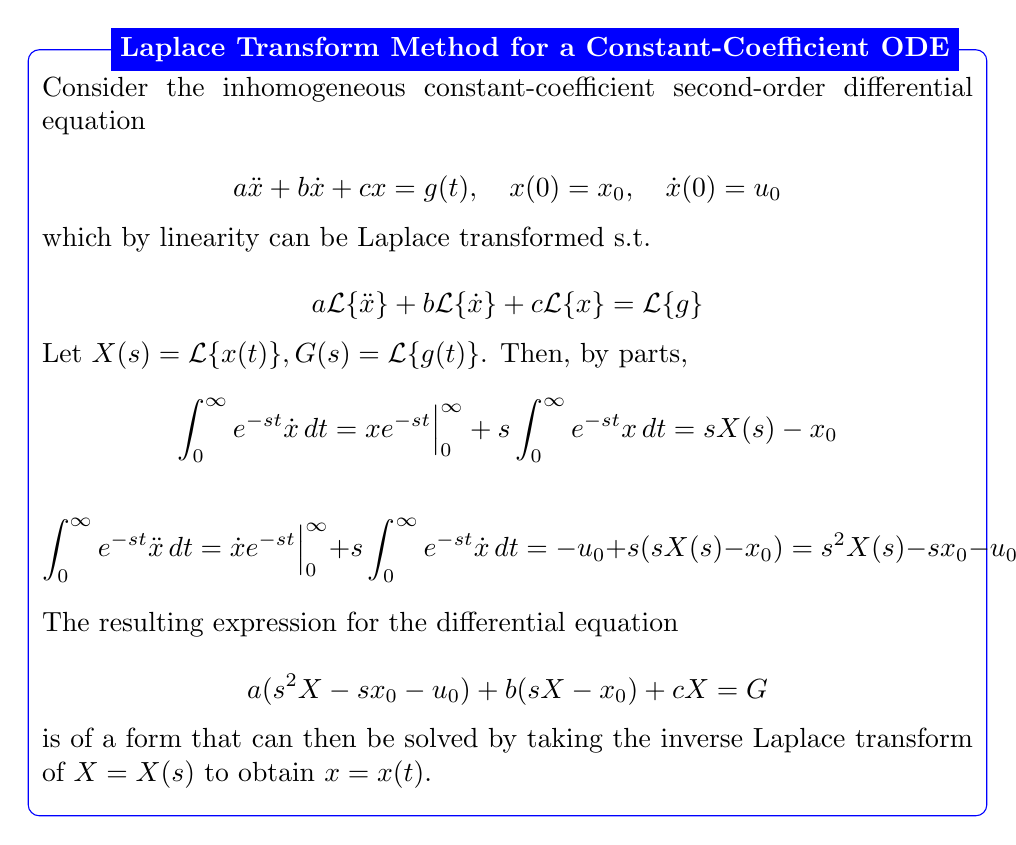
\begin{tikzpicture}
\node [rounded-box] (box){\begin{minipage}{0.975\textwidth}
    Consider the inhomogeneous constant-coefficient second-order differential equation

    $$a \ddot{x} + b \dot{x} + c x = g(t), \quad x(0) = x_0, \quad \dot{x}(0) = u_0$$

    which by linearity can be Laplace transformed s.t.

    $$a \mathcal{L}\{\ddot{x}\} + b \mathcal{L}\{\dot{x}\} + c \mathcal{L}\{x\} = \mathcal{L}\{g\}$$

    Let $X(s) = \mathcal{L}\{x(t)\}, G(s) = \mathcal{L}\{g(t)\}$. Then, by parts,

    $$\int_0^\infty e^{-st} \dot{x} \, dt = x e^{-st} \Big|_0^\infty + s \int_0^\infty e^{-st} x \, dt = s X(s) - x_0$$

    $$\int_0^\infty e^{-st} \ddot{x} \, dt = \dot{x} e^{-st} \Big|_0^\infty + s \int_0^\infty e^{-st} \dot{x} \, dt = -u_0 + s(s X(s) - x_0) = s^2 X(s) - s x_0 - u_0$$

    The resulting expression for the differential equation

    $$a(s^2 X - s x_0 - u_0) + b(s X - x_0) + c X = G$$

    is of a form that can then be solved by taking the inverse Laplace transform of $X = X(s)$ to obtain $x = x(t)$.
\end{minipage}};
\node[rounded-box-title, left=10pt] at (box.north east) {Laplace Transform Method for a Constant-Coefficient ODE};
\end{tikzpicture}

\textbf{Example}: $\ddot{x} + x = \sin{2 t}, x(0) = 2, \dot{x}(0) = 1$

Taking the Laplace transform of both sides, $s^2 X(s) - 2 s - 1 + X(s) = \frac{2}{s^2 + 4}$. Thus, $X(s) = \frac{2 s + 1}{s^2 + 1} + \frac{2}{(s^2 + 1) (s^2 + 4)}$.

To determine the inverse Laplace transform from the table, perform a partial fraction expansion of: $\frac{2}{(s^2 + 1) (s^2 + 4)} = \frac{a s + b}{s^2 + 1} + \frac{c s + d}{s^2 + 4}$.

Therefore, $a = c = 0, b = 2 / 3, d = - b$, and $X(s) = \frac{2 s + 1}{s^2 + 1} + \frac{2 / 3}{x^2 + 1} - \frac{2 / 3}{s^2 + 4} = \frac{2 s}{s^2 + 1} + \frac{5 / 3}{s^2 + 1} - \frac{2 / 3}{s^2 + 4}$.

Taking the inverse Laplace transforms of the three terms separately, where the values in the table are $b = 1$ in the first two terms, and $b = 2$ in the third term:

\vspace{-10pt}

$$x(t) = 2 \cos{t} + \frac{5}{3} \sin{t} - \frac{1}{3} \sin{2 t}$$

\subsection{The Heaviside Step Function and Dirac Delta Function}

\begin{paracol}{2}

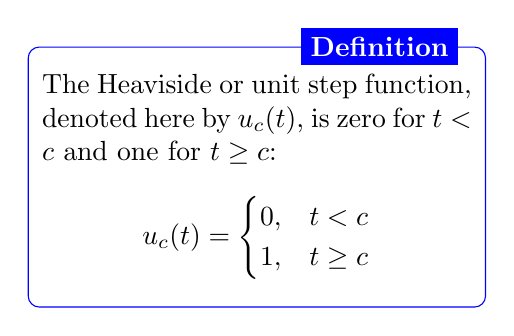
\begin{tikzpicture}
\node [rounded-box] (box){\begin{minipage}{0.45\textwidth}
    The Heaviside or unit step function, denoted here by $u_c(t)$, is zero for $t < c$ and one for $t \geq c$:

    $$u_c(t) = \begin{cases}
        0, & t < c \\
        1, & t \geq c
    \end{cases}$$
\end{minipage}};
\node[rounded-box-title, left=10pt] at (box.north east) {Definition};
\end{tikzpicture}

\switchcolumn

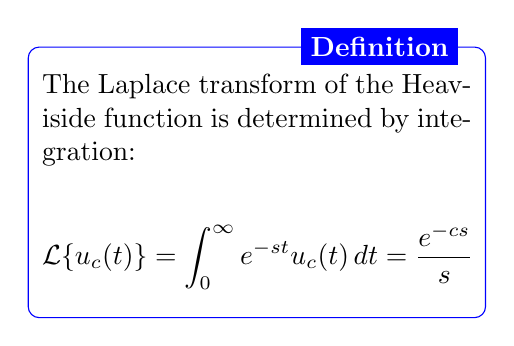
\begin{tikzpicture}
\node [rounded-box] (box){\begin{minipage}{0.45\textwidth}
    The Laplace transform of the Heaviside function is determined by integration:

    $$\mathcal{L}\{ u_c(t) \} = \int_0^\infty e^{-st} u_c(t) \, dt = \frac{e^{-cs}}{s}$$
\end{minipage}};
\node[rounded-box-title, left=10pt] at (box.north east) {Definition};
\end{tikzpicture}

\switchcolumn

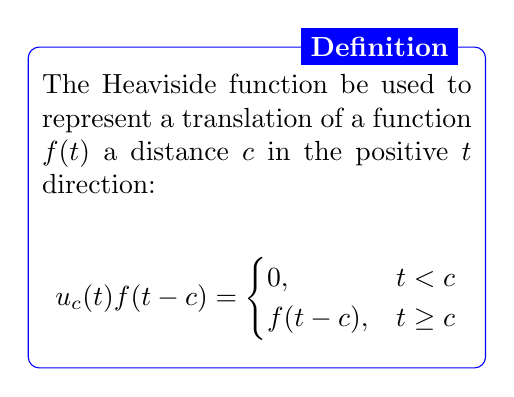
\begin{tikzpicture}
\node [rounded-box] (box){\begin{minipage}{0.45\textwidth}
    The Heaviside function be used to represent a translation of a function $f(t)$ a distance $c$ in the positive $t$ direction:

    $$u_c(t) f(t - c) = \begin{cases}
        0, & t < c \\
        f(t - c), & t \geq c
    \end{cases}$$
\end{minipage}};
\node[rounded-box-title, left=10pt] at (box.north east) {Definition};
\end{tikzpicture}

\switchcolumn

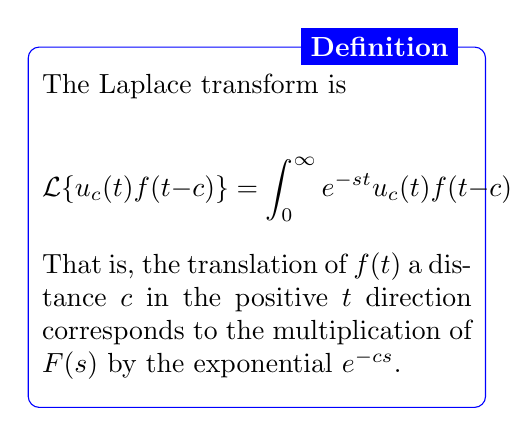
\begin{tikzpicture}
\node [rounded-box] (box){\begin{minipage}{0.45\textwidth}
    The Laplace transform is

    $$\mathcal{L}\{ u_c(t) f(t - c) \} = \int_0^\infty e^{-st} u_c(t) f(t - c) \, dt = e^{-cs} F(s)$$

    That is, the translation of $f(t)$ a distance $c$ in the positive $t$ direction corresponds to the multiplication of $F(s)$ by the exponential $e^{-cs}$.
\end{minipage}};
\node[rounded-box-title, left=10pt] at (box.north east) {Definition};
\end{tikzpicture}

\end{paracol}

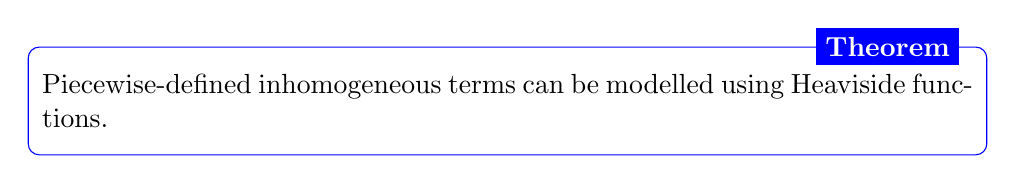
\begin{tikzpicture}
\node [rounded-box] (box){\begin{minipage}{0.975\textwidth}
    Piecewise-defined inhomogeneous terms can be modelled using Heaviside functions.
\end{minipage}};
\node[rounded-box-title, left=10pt] at (box.north east) {Theorem};
\end{tikzpicture}

\textbf{Example}: Consider the general case of a piecewise function defined on two intervals:

$$f(t) = \begin{cases}
    f_1(t), & \text{if } t < c \\
    f_2(t), & \text{if } t \geq c
\end{cases}$$

Using the Heaviside function $u_c$, the function $f(t)$ can be written in a single line as

$$f(t) = f_1(t) + \big( f_2(t) - f_1(t) \big) u_c(t)$$

\begin{paracol}{2}

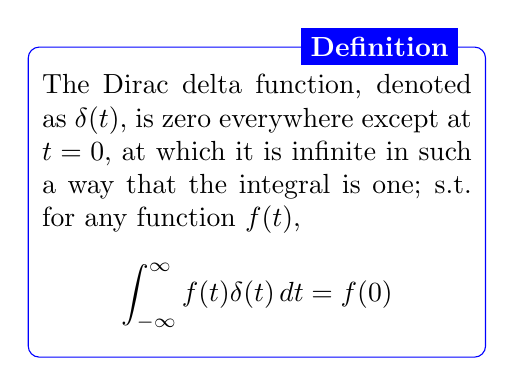
\begin{tikzpicture}
\node [rounded-box] (box){\begin{minipage}{0.45\textwidth}
    The Dirac delta function, denoted as $\delta(t)$, is zero everywhere except at $t = 0$, at which it is infinite in such a way that the integral is one; s.t. for any function $f(t)$,

    $$\int_{-\infty}^\infty f(t) \delta(t) \, dt = f(0)$$
\end{minipage}};
\node[rounded-box-title, left=10pt] at (box.north east) {Definition};
\end{tikzpicture}

\switchcolumn

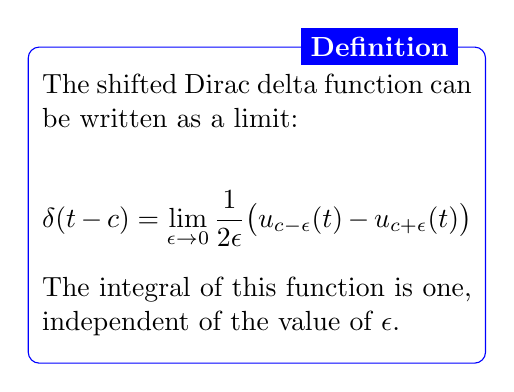
\begin{tikzpicture}
\node [rounded-box] (box){\begin{minipage}{0.45\textwidth}
    The shifted Dirac delta function can be written as a limit:

    $$\delta(t - c) = \lim_{\epsilon \rightarrow 0} \frac{1}{2 \epsilon} \big(u_{c - \epsilon}(t) - u_{c+\epsilon}(t)\big)$$

    The integral of this function is one, independent of the value of $\epsilon$.
\end{minipage}};
\node[rounded-box-title, left=10pt] at (box.north east) {Definition};
\end{tikzpicture}

\end{paracol}

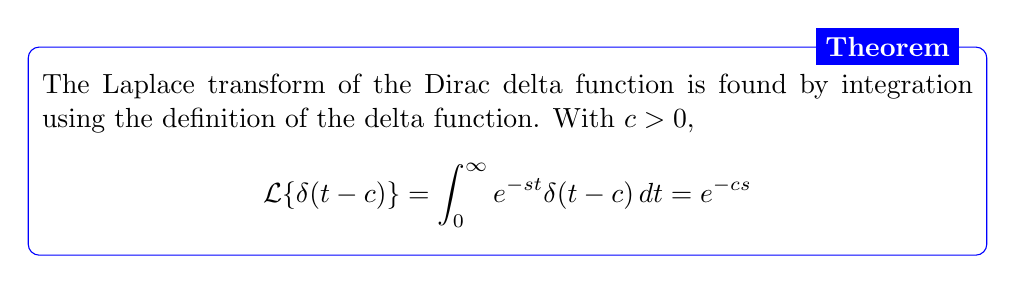
\begin{tikzpicture}
\node [rounded-box] (box){\begin{minipage}{0.975\textwidth}
    The Laplace transform of the Dirac delta function is found by integration using the definition of the delta function. With $c > 0$,

    $$\mathcal{L}\{ \delta(t - c) \} = \int_0^\infty e^{-st} \delta(t - c) \, dt = e^{-cs}$$
\end{minipage}};
\node[rounded-box-title, left=10pt] at (box.north east) {Theorem};
\end{tikzpicture}

\textbf{Example}: Solution of a discontinuous inhomogeneous term: $\ddot{x} + 3 \dot{x} + 2 x = 1 - u_1(t), x(0) = \dot{x}(0) = 0$

The inhomogeneous term is a step-down function, from one to zero.

Taking the Laplace transform, $s^2 X(s) + 3 s X(s) + 2 X(s) = \frac{1}{s} (1 - e^{-s})$ with solution for $X = X(s)$ given by $X(s) = \frac{1 - e^{-s}}{s(s+1)(s+2)}$.

Defining $F(s) = \frac{1}{s(s+1)(s+2)}$, the inverse Laplace transform of $X(s)$ can be written as $x(t) = f(t) - u_1(t) f(t - 1)$, where $f(t)$ is the inverse Laplace transform of $F(s)$.

To determine $f(t)$, the partial fraction expansion of $F(s)$ is $\frac{1}{s(s+1)(s+2)} = \frac{a}{s} + \frac{b}{s+1} + \frac{c}{s+2}$ with $a = 1 / 2, b = -1, c -= 1 / 2$.

$$\mathcal{L}^{-1}\{ F(s) \} = \frac{1}{2} \mathcal{L}^{-1} \Big\{ \frac{1}{s} \Big\} - \mathcal{L}^{-1} \Big\{ \frac{1}{s+1} \Big\} + \frac{1}{2} \mathcal{L}^{-1} \Big\{ \frac{1}{s+2} \Big\} = \frac{1}{2} - e^{-t} + \frac{1}{2} e^{-2t}$$

$$x(t) = \frac{1}{2} - e^{-t} + \frac{1}{2} e^{-2t} - u_1(t) \Big( \frac{1}{2} - e^{-(t-1)} + \frac{1}{2} e^{-2(t-1)} \Big)$$

\subsection{The Series Solution Method}

\textbf{Example}: $y'' + y = 0$

$$
y(x) = \sum_{n=0}^\infty a_n x^n
\qquad
y'(x) = \sum_{n=1}^\infty n a_n x^{n-1}
\qquad
y''(x) = \sum_{n=2}^\infty n (n-1) a_n x^{n-2}
$$

$$\sum_{n=2}^\infty n (n-1) a_n x^{n-2} + \sum_{n=1}^\infty n a_n x^{n-1} = 0$$

$$\sum_{n=0}^\infty (n+2)(n+1) a_{n+2} x^n + \sum_{n=1}^\infty n a_n x^{n-1} = 0$$

$$\sum_{n=0}^\infty \big( (n+2) (n+1) a_{n+2} + a_n \big) x^n = 0$$

For the equality to hold, the coefficient of each power of $x$ must vanish separately. Therefore,

$$a_{n+2} = - \frac{a_n}{(n+2)(n+1)}, n = 0, 1, 2, \dots$$

Even and odd coefficients decouple. Thus, there are two independent sequences:

$$a_0, \quad a_2 = - \frac{1}{2}a_0, \quad a_4 = - \frac{1}{d \cdot 3} a_2 = \frac{1}{4!} a_0, \quad \dots$$

$$a_1, \quad a_3 = - \frac{1}{3 \cdot 2} a_1, \quad a_5 = - \frac{1}{5 \cdot 4} a_3 = \frac{1}{5!} a_1, \quad \dots$$

By the principle of superposition, the general is

\begin{align*}
    y(x) & = a_0 \Big( 1 - \frac{x^2}{2!} + \frac{x^4}{4!} - \dots \Big) + a_1 \Big( x - \frac{x^3}{3!} + \frac{x^5}{5!} - \dots \Big) \\
    & = a_0 \cos{x} + a_1 \sin{x}
\end{align*}
 \newpage
\section{Systems of Differential Equations}

More than one dependent variables $x_1, x_2, \dots$ give rise to a system of differential equations.

\subsection{Eigenvalues and Eigenvectors}

The eigenvalue problem for an $n \times n$ matrix $A$ is given by

$$A \mathbf{x} = \lambda x \quad \iff \quad (A - \lambda I) \mathbf{x} = \mathbf{0}$$

where the scalar $\lambda$ is called the eigenvalue and the $n \times 1$ column vector $x$ is called the eigenvector.

When $A$ is a $2 \times 2$ matrix, then

$$A - \lambda I = \begin{pmatrix}
    a_{11} - \lambda & a_{12} \\
    a_{21} & a_{22} - \lambda
\end{pmatrix}$$

A solution other than $\mathbf{x} = \mathbf{0}$ of the eigenvalue equation exists provided

$$\det(A - \lambda I) = 0$$

This equation is called the characteristic equation of $A$, and is given by

$$\lambda^2 - (a_{11} + a_{22}) \lambda + (a_{11} a_{22} - a_{12} a_{21}) = 0$$

$$\lambda^2 - \text{Tr}(A) \lambda + \det(A) = 0$$

The eigenvalues can be real and distinct, complex conjugates, or repeated.

After determining an eigenvalue, say $\lambda = \lambda_1$, the corresponding eigenvector $\mathbf{v}_1$ can be found by solving

$$(A - \lambda_1 I) \mathbf{v}_1 = \mathbf{0}$$

\subsection{Systems of First-Order Linear Ordinary Differential Equations}

\begin{paracol}{2}

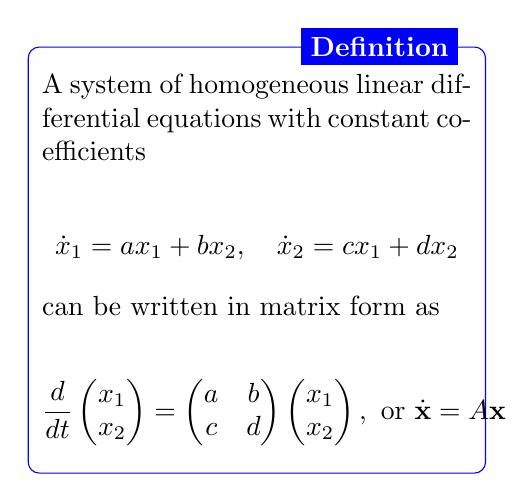
\begin{tikzpicture}
\node [rounded-box] (box){\begin{minipage}{0.45\textwidth}
    A system of homogeneous linear differential equations with constant coefficients

    $$\dot{x}_1 = a x_1 + b x_2, \quad \dot{x}_2 = c x_1 + d x_2$$

    can be written in matrix form as

    $$\frac{d}{dt}\begin{pmatrix}
        x_1 \\ x_2
    \end{pmatrix} = \begin{pmatrix}
        a & b \\
        c & d
    \end{pmatrix} \begin{pmatrix}
        x_1 \\ x_2
    \end{pmatrix}, \text{ or } \dot{\mathbf{x}} = A \mathbf{x}$$
\end{minipage}};
\node[rounded-box-title, left=10pt] at (box.north east) {Definition};
\end{tikzpicture}

\switchcolumn

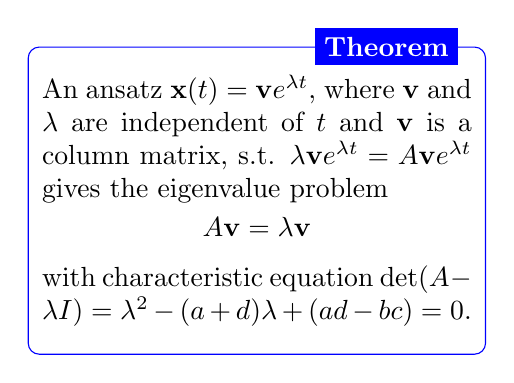
\begin{tikzpicture}
\node [rounded-box] (box){\begin{minipage}{0.45\textwidth}
    An ansatz $\mathbf{x}(t) = \mathbf{v} e^{\lambda t}$, where $\mathbf{v}$ and $\lambda$ are independent of $t$ and $\mathbf{v}$ is a column matrix, s.t. $\lambda \mathbf{v} e^{\lambda t} = A \mathbf{v} e^{\lambda t}$ gives the eigenvalue problem

    \vspace{-10pt}

    $$A \mathbf{v} = \lambda \mathbf{v}$$

    with characteristic equation $\det(A - \lambda I) = \lambda^2 - (a + d) \lambda + (ad - bc) = 0$.
\end{minipage}};
\node[rounded-box-title, left=10pt] at (box.north east) {Theorem};
\end{tikzpicture}

\switchcolumn

\textbf{Example}: $\dot{x}_1 = x_1 + x_2, \dot{x}_2 = 4 x_1 + x_2$

With the ansatz $\mathbf{x}(t) = \mathbf{v} e^{\lambda t}$,

$$\det(A - \lambda I) = \lambda^2 - 2 \lambda - 3 = (\lambda -3) (\lambda + 1) = 0$$

and the eigenvalues and eigenvectors are

$$\lambda_1 = -1, \quad \mathbf{v} = \begin{pmatrix}
    1 \\ -2
\end{pmatrix}, \quad \lambda_2 = 3, \quad \mathbf{v}_2 = \begin{pmatrix}
    1 \\ 2
\end{pmatrix}$$

By the principle of superposition,

$$x(t) = c_1 v_1 e^{\lambda_1 t} + c_2 v_2 e^{\lambda_2 t}$$

or explicitly writing out the components,

$$x_1(t) = c_1 e^{-t} + c_2 e^{3t}, \quad x_2(t) = -2 c_1 e^{-t} + 2 c_2 e^{3t}$$

\switchcolumn

\textbf{Example}: $\dot{x}_1 = - \frac{1}{2} x_1 + x_2, \dot{x}_2 = - x_1 - \frac{1}{2} x_2$

With the ansatz $\mathbf{x}(t) = \mathbf{v} e^{\lambda t}$, the characteristic equation is $\det(A - \lambda I) = \lambda^2 + \lambda + \frac{5}{4} = 0$, which has \textbf{complex-conjugate roots}: $\lambda = - \frac{1}{2} + i, \quad \bar{\lambda} = - \frac{1}{2} - i$.

We can form a linear combination of the two complex eigenvectors $\mathbf{v} e^{\lambda t}, \bar{\mathbf{v}} e^{\lambda t}$ to construct two independent real solutions:

$$\text{Re}\{ \mathbf{v} e^{\lambda t} \} = \text{Re}\{ \begin{pmatrix}
    1 \\ i
\end{pmatrix} e^{(-\frac{1}{2} + i)t} \} = e^{-t / 2} \begin{pmatrix}
    \cos{t} & - \sin{t}
\end{pmatrix}$$

$$\text{Im}\{ \mathbf{v} e^{\lambda t} \} = \text{Im}\{ \begin{pmatrix}
    1 \\ i
\end{pmatrix} e^{(-\frac{1}{2} + i)t} \} = e^{-t / 2} \begin{pmatrix}
    \sin{t} & \cos{t}
\end{pmatrix}$$

Taking a linear superposition of these two real solutions,

$$\mathbf{x}(t) = e^{-t / 2} \Bigg( A \begin{pmatrix}
    \cos{t} \\ - \sin{t}
\end{pmatrix} + B \begin{pmatrix}
    \sin{t} \\ \cos{t}
\end{pmatrix} \Bigg)$$

\end{paracol}

\subsection{Phase Portraits}

\begin{paracol}{2}

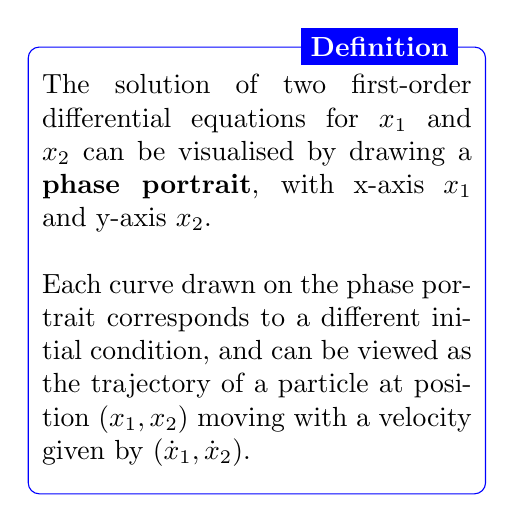
\begin{tikzpicture}
\node [rounded-box] (box){\begin{minipage}{0.45\textwidth}
    The solution of two first-order differential equations for $x_1$ and $x_2$ can be visualised by drawing a \textbf{phase portrait}, with x-axis $x_1$ and y-axis $x_2$. \\

    Each curve drawn on the phase portrait corresponds to a different initial condition, and can be viewed as the trajectory of a particle at position $(x_1, x_2)$ moving with a velocity given by $(\dot{x}_1, \dot{x}_2)$.
\end{minipage}};
\node[rounded-box-title, left=10pt] at (box.north east) {Definition};
\end{tikzpicture}

\switchcolumn

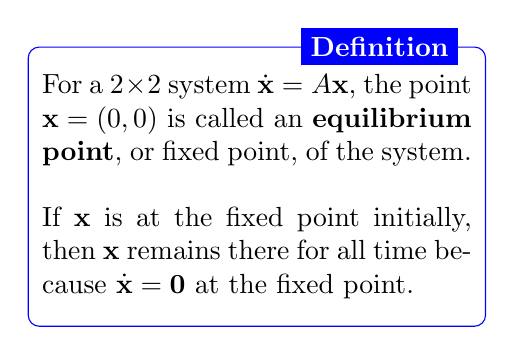
\begin{tikzpicture}
\node [rounded-box] (box){\begin{minipage}{0.45\textwidth}
    For a $2 \times 2$ system $\dot{\mathbf{x}} = A \mathbf{x}$, the point $\mathbf{x} = (0, 0)$ is called an \textbf{equilibrium point}, or fixed point, of the system. \\

    If $\mathbf{x}$ is at the fixed point initially, then $\mathbf{x}$ remains there for all time because $\dot{\mathbf{x}} = \mathbf{0}$ at the fixed point.
\end{minipage}};
\node[rounded-box-title, left=10pt] at (box.north east) {Definition};
\end{tikzpicture}

\switchcolumn

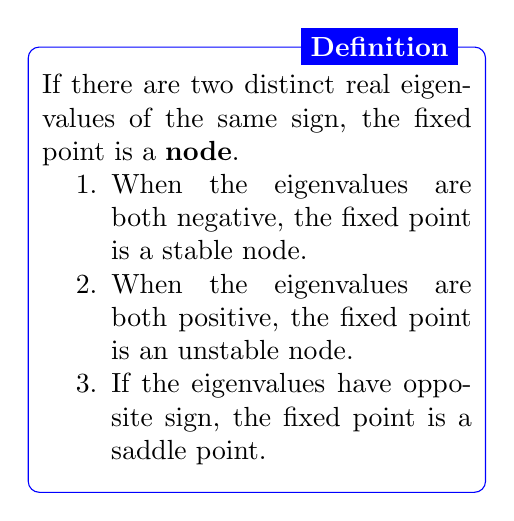
\begin{tikzpicture}
\node [rounded-box] (box){\begin{minipage}{0.45\textwidth}
    If there are two distinct real eigenvalues of the same sign, the fixed point is a \textbf{node}.

    \begin{enumerate}
        \item When the eigenvalues are both negative, the fixed point is a stable node.
        \item When the eigenvalues are both positive, the fixed point is an unstable node.
        \item If the eigenvalues have opposite sign, the fixed point is a saddle point.
    \end{enumerate}
\end{minipage}};
\node[rounded-box-title, left=10pt] at (box.north east) {Definition};
\end{tikzpicture}

\switchcolumn

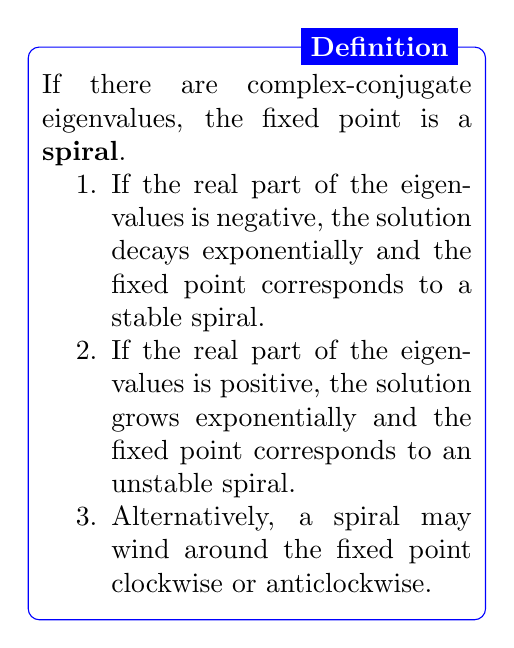
\begin{tikzpicture}
\node [rounded-box] (box){\begin{minipage}{0.45\textwidth}
    If there are complex-conjugate eigenvalues, the fixed point is a \textbf{spiral}.

    \begin{enumerate}
        \item If the real part of the eigenvalues is negative, the solution decays exponentially and the fixed point corresponds to a stable spiral.
        \item If the real part of the eigenvalues is positive, the solution grows exponentially and the fixed point corresponds to an unstable spiral.
        \item Alternatively, a spiral may wind around the fixed point clockwise or anticlockwise.
    \end{enumerate}
\end{minipage}};
\node[rounded-box-title, left=10pt] at (box.north east) {Definition};
\end{tikzpicture}

\switchcolumn

\textbf{Example}: Consider the differential equations given by $\dot{x}_1 = -3 x_1 + \sqrt{2} x_2, \dot{x}_2 = \sqrt{2} x_1 - 2 x_2$. This system has eigenvalues and eigenvectors $\lambda_1 = -4, \mathbf{v}_1 = \begin{pmatrix}
    1 \\ - \sqrt{2} / 2
\end{pmatrix}, \lambda_2 = -1, \mathbf{v}_2 = \begin{pmatrix}
    1 \\ \sqrt{2}
\end{pmatrix}$.

Because $\lambda_1, 
\lambda_2 < 0$, both exponential solutions for $\mathbf{x} = \mathbf{x}(t)$ decay in time and $\mathbf{x} \rightarrow (0, 0)$ as $t \rightarrow \infty$.

The node is stable.

\textbf{Example}: Consider the differential equations given by $\dot{x}_1 = x_1 + x_2, \dot{x}_2 = 4 x_1 + x_2$. This system has eigenvalues and eigenvectors $\lambda_1 = -1, \mathbf{v}_1 = \begin{pmatrix}
    1 \\ - 2
\end{pmatrix}, \lambda_2 = 3, \mathbf{v}_2 = \begin{pmatrix}
    1 \\ 2
\end{pmatrix}$.

Because $\lambda_1 < 0$, trajectories approach the fixed point along the direction of the first eigenvector, and because $\lambda_2 > 0$, trajectories move away from the fixed point along the direction of the second eigenvector.

Ultimately, a saddle point is an unstable equilibrium because for any initial conditions such that $c_2 \neq 0, |x(t)| \rightarrow \infty$ as $t \rightarrow \infty$.

The node is stable.

\switchcolumn

\textbf{Example}: Consider the system of differential equations given by $x_1 = - \frac{1}{2} x_1 + x_2, \quad x_2 = - x_1 - \frac{1}{2} x_2$. This system has complex eigenvalue and eigenvector

$$\lambda = - \frac{1}{2} + i, \mathbf{v} = \begin{pmatrix}
    1 \\ i
\end{pmatrix},$$

and their complex conjugates.

The general solution is written as

$$\mathbf{x}(t) = e^{-t / 2} \Bigg[ A \begin{pmatrix}
    \cos{t} \\ - \sin{t}
\end{pmatrix} + B \begin{pmatrix}
    \sin{t} \\ \cos{t}
\end{pmatrix} \Bigg]$$

The trajectories in the phase portrait are spirals centred at the fixed point.

If $\text{Re}(\lambda) > 0$, the trajectories spiral out; if $\text{Re}(\lambda) < 0$, they spiral in.

The spirals around the fixed point may be clockwise or counterclockwise, depending on the governing equations.

Here, since $\text{Re}(\lambda) = -1/2 < 0$, the trajectories spiral into the origin.

To determine whether the spiral is
clockwise or counterclockwise, examine the time derivatives at the point $(x_1, x_2) = (0, 1)$.

At this point in the phase space, $(x_1, x_2) = (1, - 1/2)$, and a particle on this trajectory moves to the right and downward, indicating a clockwise spiral. 

\end{paracol}

\subsection{Normal Modes}

\begin{paracol}{2}

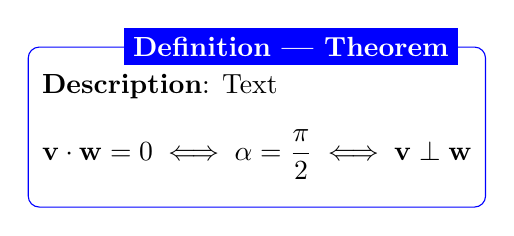
\begin{tikzpicture}
\node [rounded-box] (box){\begin{minipage}{0.45\textwidth}
    \textbf{Description}: Text
    $$\mathbf{v} \cdot \mathbf{w} = 0 \iff \alpha = \frac{\pi}{2} \iff \mathbf{v} \perp \mathbf{w}$$
\end{minipage}};
\node[rounded-box-title, left=10pt] at (box.north east) {Definition | Theorem};
\end{tikzpicture}

\end{paracol}

\newpage

\subsection{Modelling with Differential Equations}

\begin{paracol}{2}

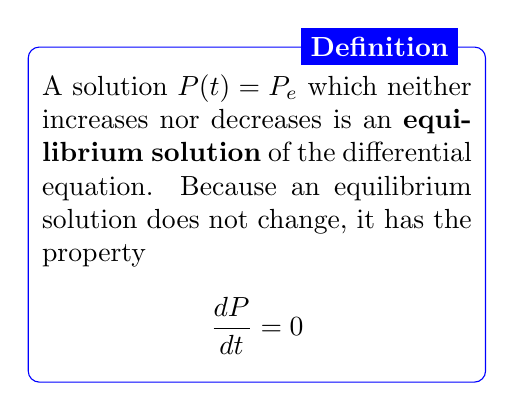
\begin{tikzpicture}
\node [rounded-box] (box){\begin{minipage}{0.45\textwidth}
    A solution $P(t) = P_e$ which neither increases nor decreases is an \textbf{equilibrium solution} of the differential equation. Because an equilibrium solution does not change, it has the property
    
    $$\frac{dP}{dt} = 0$$
\end{minipage}};
\node[rounded-box-title, left=10pt] at (box.north east) {Definition};
\end{tikzpicture}

In other words, the equilibrium solution is constant in time.

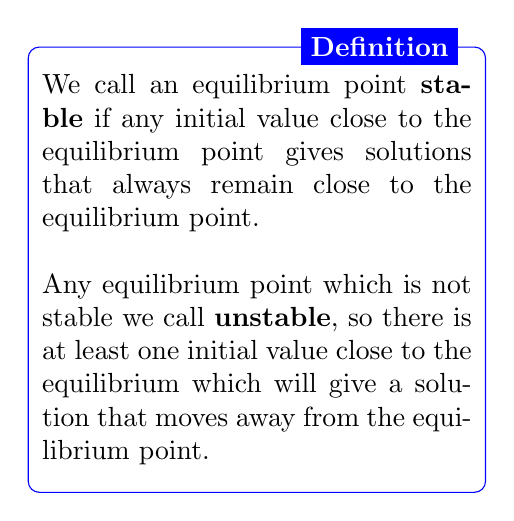
\begin{tikzpicture}
\node [rounded-box] (box){\begin{minipage}{0.45\textwidth}
    We call an equilibrium point \textbf{stable} if any initial value close to the equilibrium point gives solutions that always remain close to the equilibrium point. \\
    
    Any equilibrium point which is not stable we call \textbf{unstable}, so there is at least one initial value close to the equilibrium which will give a solution that moves away from the equilibrium point.
\end{minipage}};
\node[rounded-box-title, left=10pt] at (box.north east) {Definition};
\end{tikzpicture}

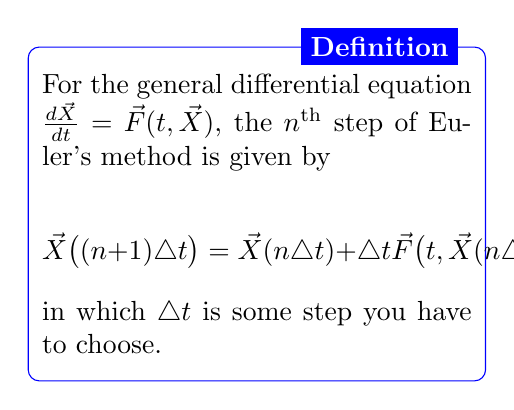
\begin{tikzpicture}
\node [rounded-box] (box){\begin{minipage}{0.45\textwidth}
    For the general differential equation $\frac{d\vec{X}}{dt} = \vec{F}(t, \vec{X})$, the $n^\text{th}$ step of Euler's method is given by

    $$\vec{X}\big((n+1) \triangle t\big) = \vec{X}(n \triangle t) + \triangle t \vec{F}\big(t, \vec{X}(n \triangle t)\big)$$

    in which $\triangle t$ is some step you have to choose.
\end{minipage}};
\node[rounded-box-title, left=10pt] at (box.north east) {Definition};
\end{tikzpicture}

\switchcolumn

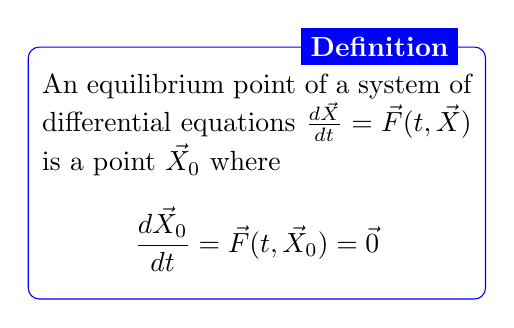
\begin{tikzpicture}
\node [rounded-box] (box){\begin{minipage}{0.45\textwidth}
    An equilibrium point of a system of differential equations $\frac{d\vec{X}}{dt} = \vec{F}(t, \vec{X})$ is a point $\vec{X}_0$ where

    $$\frac{d\vec{X}_0}{dt} = \vec{F}(t, \vec{X}_0) = \vec{0}$$
\end{minipage}};
\node[rounded-box-title, left=10pt] at (box.north east) {Definition};
\end{tikzpicture}

\begin{itemize}
    \item An equilibrium point $\vec{X}_0$ is called a saddle point if the Jacobian matrix $J(\vec{X}_0)$ has one negative and one positive eigenvalue.

    \item An equilibrium point $\vec{X}_0$ is called a stable node if the Jacobian matrix $J(\vec{X}_0)$ has two negative eigenvalues: all solutions that start near the equilibrium point stay near the equilibrium point.

    \item An equilibrium point $\vec{X}_0$ is called an unstable node if the Jacobian matrix $J(\vec{X}_0)$ has two positive eigenvalues: all solutions that start near the equilibrium point stay near the equilibrium point.

    \item An equilibrium point $\vec{X}_0$ is called a stable spiral point if the Jacobian matrix $J(\vec{X}_0)$ has two complex eigenvalues $\lambda = a \pm bi$ with negative real parts: $a < 0$.

    \item An equilibrium point $\vec{X}_0$ is called an unstable spiral point if the Jacobian matrix $J(\vec{X}_0)$ has two complex eigenvalues $\lambda = a \pm bi$ with positive real parts: $a > 0$.

    \item An equilibrium point $\vec{X}_0$ is called a circle point if the Jacobian matrix $J(\vec{X}_0)$ has two complex eigenvalues with zero real parts:  $\lambda = \pm bi$.
\end{itemize}

\end{paracol}
 \newpage
\section{Partial Differential Equations}

Differential equations with more than one independent variables $x, y, \dots$ s.t. $f = f(x, y, \dots)$ are partial differential equations.

\subsection{Fourier Series}

\begin{paracol}{2}

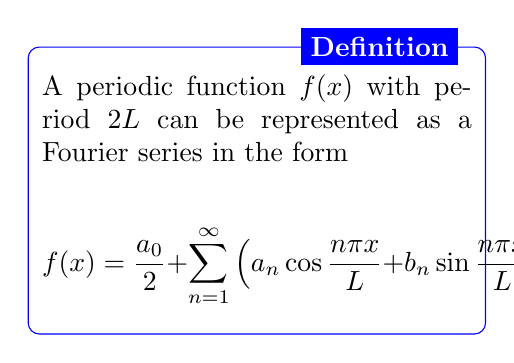
\begin{tikzpicture}
\node [rounded-box] (box){\begin{minipage}{0.45\textwidth}
    A periodic function $f(x)$ with period $2L$ can be represented as a Fourier series in the form

    $$f(x) = \frac{a_0}{2} + \sum_{n=1}^\infty \Big( a_n \cos{\frac{n \pi x}{L}} + b_n \sin{\frac{n \pi x}{L}}$$
\end{minipage}};
\node[rounded-box-title, left=10pt] at (box.north east) {Definition};
\end{tikzpicture}

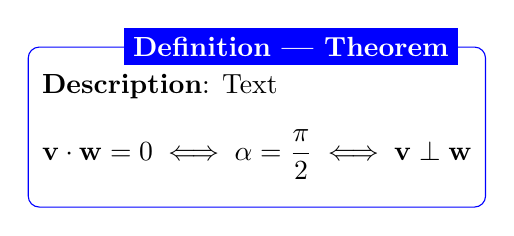
\begin{tikzpicture}
\node [rounded-box] (box){\begin{minipage}{0.45\textwidth}
    \textbf{Description}: Text
    $$\mathbf{v} \cdot \mathbf{w} = 0 \iff \alpha = \frac{\pi}{2} \iff \mathbf{v} \perp \mathbf{w}$$
\end{minipage}};
\node[rounded-box-title, left=10pt] at (box.north east) {Definition | Theorem};
\end{tikzpicture}

\end{paracol}

\subsection{The Diffusion Equation}

\begin{paracol}{2}

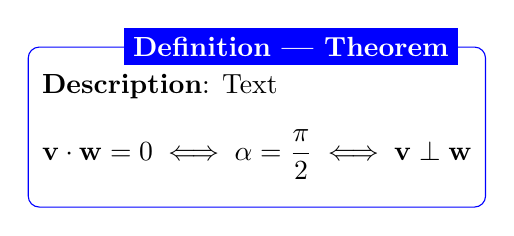
\begin{tikzpicture}
\node [rounded-box] (box){\begin{minipage}{0.45\textwidth}
    \textbf{Description}: Text
    $$\mathbf{v} \cdot \mathbf{w} = 0 \iff \alpha = \frac{\pi}{2} \iff \mathbf{v} \perp \mathbf{w}$$
\end{minipage}};
\node[rounded-box-title, left=10pt] at (box.north east) {Definition | Theorem};
\end{tikzpicture}

\end{paracol}
 \newpage

\nocite{*}
\printbibliography

\end{document}
